\documentclass[9pt]{extarticle}
\usepackage[a4paper,margin=0.25in]{geometry}
\usepackage{lmodern}
\usepackage{multicol}
\usepackage{amsmath,amssymb}
\usepackage{graphicx}
\usepackage{tikz}
\usepackage{polynom}
\usepackage{enumitem}
\usepackage{titlesec}
\usepackage[dvipsnames]{xcolor}
\usepackage{tcolorbox}
\tcbuselibrary{skins,breakable}
\usepackage{fancyhdr}
\pagestyle{fancy}
\fancyhf{}
\renewcommand{\headrulewidth}{0pt}
\setlength{\parindent}{0pt}
\setlength{\columnsep}{0.15in}
\setlength{\columnseprule}{0.4pt}
\setlength{\abovedisplayskip}{2pt}
\setlength{\belowdisplayskip}{2pt}
\setlength{\abovedisplayshortskip}{1pt}
\setlength{\belowdisplayshortskip}{1pt}
\allowdisplaybreaks
\emergencystretch=2em

\setlist[itemize]{itemsep=0.5pt,parsep=0pt,topsep=1pt,leftmargin=*,partopsep=0pt}
\setlist[enumerate]{itemsep=0.5pt,parsep=0pt,topsep=1pt,leftmargin=*,partopsep=0pt}

\titleformat{\section}{\normalfont\bfseries\small\color{RoyalBlue}}{\thesection}{0.3em}{\titlerule[0.9pt]}
\titlespacing{\section}{0pt}{4pt}{2pt}
\titleformat{\subsection}{\normalfont\bfseries\footnotesize\color{OliveGreen}}{}{0em}{}
\titlespacing{\subsection}{0pt}{2pt}{1.5pt}
\setlength{\parskip}{0.5pt}

\newcommand{\hl}[1]{\textbf{\textcolor{BrickRed}{#1}}}
\newcommand{\sepline}{\vspace{1pt}{\color{RoyalBlue}\hrule}\vspace{3pt}}

\newtcolorbox{kbox}{colback=RoyalBlue!10,colframe=RoyalBlue!70,boxrule=0.6pt,arc=1.5pt,left=1.5pt,right=1.5pt,top=1pt,bottom=1pt,boxsep=0pt}
\newtcolorbox{obox}{colback=Apricot!25,colframe=Orange!85!black,boxrule=0.6pt,arc=1.5pt,left=1.5pt,right=1.5pt,top=1pt,bottom=1pt,boxsep=0pt}

\begin{document}
\footnotesize

\begin{center}
\colorbox{RoyalBlue!15}{\parbox{0.97\linewidth}{\centering
{\bfseries\large\color{RoyalBlue} Computer Algebra (SCI19 3112) --- Midterm Cheat Sheet}\\[1.5pt]
{\scriptsize\color{RoyalBlue!70!black} Numbers $\cdot$ Two's-complement / IEEE754 $\cdot$ GCD / APN / Prime-fact $\cdot$ Trees / Rewrites $\cdot$ Modular / Poly-mod $\cdot$ Groups / FLT}}}
\end{center}
\sepline

\begin{multicols}{3}

\section{Prof's Blueprint (High Priority)}
\hl{Exam:} MCQ + written, \hl{30 pts total}. Practical (worked-number) problems dominate; fewer theory questions. Calculator allowed; \hl{no programming} required. One A4 sheet allowed (this one).
\hl{Highest-frequency tools:} dec$\leftrightarrow$bin, two's complement, IEEE 754, gcd, mod arithmetic + tables, inverses/zero divisors, poly-mod reduction, group axioms/order/Lagrange, FLT big powers, expression trees + Lisp lists, substitution vs rewrite.

\section{Sets \& Exact vs Approximate}
$\mathbb N$: here \hl{$\{1,2,3,\ldots\}$ (no 0!)}; $\mathbb Z=\{0,\pm1,\pm2,\ldots\}$; $\mathbb Q=\{p/q:p\in\mathbb Z,\ q\ne0\}$; $\mathbb R$; $\mathbb Z[x]$ = polynomials with integer coefficients.
\hl{Prime:} integer $>1$ with exactly 2 positive divisors (1, itself). \hl{Composite:} $>1$, more than 2 divisors. \hl{1 is neither}; 2 is the only even prime.
\hl{Exact} = symbolic: fractions kept as reduced pairs, radicals/$\pi$ kept symbolically, arbitrary precision. \hl{Approximate} = floats: rounding errors accumulate; floats \hl{cannot} represent $0.1$ exactly (repeating binary). Exact CAS features: no round-off, results provably correct, may be slow/huge.

\section{Integers in Memory (Two's Complement)}
\hl{Unsigned $n$ bits:} range $0\ldots2^n{-}1$ (max $=2^n{-}1$).
\begin{kbox}\raggedright
\textbf{Signed $n$ bits:} range $\textcolor{BrickRed}{-2^{n-1}\ldots2^{n-1}{-}1}$ (one extra negative); MSB $=1$ means negative. \textbf{Negate} $=$ flip bits ${}+1$: $-62$ (7-bit): $0111110\to1000001\to1000010_2$. \textbf{Back:} MSB $1\Rightarrow$ negate: $1111011\to0000101{=}5\Rightarrow-5$. \hl{$-2^{n-1}=100\ldots0$ has no positive counterpart.}
\end{kbox}
\hl{Bits needed for $-m$:} smallest $n$ with $2^{n-1}\ge m$: $-200\to n{=}9$ ($2^8{=}256$), $-300\to n{=}10$, $-1030\to n{=}12$, $-2{\times}10^9\to n{=}32$.
\hl{Min/max in $n$ bits:} 8-bit: unsigned $0..255$, signed $-128..127$; 16-bit signed: $-32768..32767$; 32-bit: $\pm2^{31}$ bounds.
\hl{Arithmetic:} add = bitwise with carry ($1010_2+0111_2=10001_2=17$); multiply = shift-and-add ($1010_2{\times}11_2=11110_2=30$). Shifts: $x\ll k=x\cdot2^k$, $x\gg k=x\,\mathrm{div}\,2^k$ (integer only).

\subsection{Dec$\leftrightarrow$Bin}
\textbf{Int ($\div2$, remainders bottom-up):} $21_{10}=10101_2$; $33_{10}=100001_2$; $26_{10}=11010_2$; $205_{10}=11001101_2$. \textbf{Bin$\to$dec:} $1011_2=8+2+1=11$.
\textbf{Frac ($\times2$, take integer part):} $0.6875\to0.1011_2$; $0.1_{10}=0.00011\ldots_2$ (\hl{periodic}); $0.1011_2=\frac12+\frac18+\frac1{16}=\frac{11}{16}=0.6875$.
\textbf{Mixed:} $21.09375=10101.00011_2$ ($0.09375=\frac1{16}+\frac1{32}=\frac3{32}$).

\section{IEEE 754 Floats}
Normalized: $\textcolor{BrickRed}{(-1)^s(1.f)_2\,2^{e}}$, stored with bias: value $=(-1)^s(1.f)_2\,2^{E-\mathrm{bias}}$, $\mathrm{bias}=127$ (single)/$1023$ (double). Layout: \hl{float 1+8+23}, \hl{double 1+11+52} bits.
\hl{Convert dec$\to$float:} dec$\to$bin $\to$ normalize to $1.f\times2^e$ $\to$ store $s$, fraction bits (drop leading 1), $E=e+\mathrm{bias}$.
\textbf{Worked:} $21.09375=1.010100011_2\times2^4$ $\Rightarrow s{=}0,\ f{=}010100011,\ e{=}4$; single-precision $E=4+127=131=10000011_2$.
\hl{Bin$\to$dec:} sum $2^{-k}$ place values: $0.1011_2=0.6875$.
\hl{Zero:} \hl{cannot} arise as $1.f\times2^e$ ($1.f\ne0$); IEEE reserves all-0 exponent bits for $+0,-0$. \hl{$\times$/$\div$ by 2} = exponent shift; $0.1+0.2$ gives rounding error.
\begin{obox}\raggedright
\textbf{Special bit patterns:} $\pm0$: exponent $=$ mantissa $=0$ (sign bit only); subnormal: exponent $=0$, mantissa $\ne0$; $\pm\infty$: exponent $=$ all 1s, mantissa $=0$; NaN: exponent $=$ all 1s, mantissa $\ne0$.
\end{obox}
\textbf{Range Qs (bias $=24$, 16 bits: $1+5+10$, $E\ge0$):} largest $=1.99902\times2^{31-24}=255.875$; smallest positive $=1.0\times2^{-24}\approx5.96046\times10^{-8}$; negatives mirror.

\section{GCD, Fractions, Coprime}
Division: $a=bq+r$, $0\le r<b$ ($q=a\,\mathrm{div}\,b$, $r=a\bmod b$).
\hl{Euclid:} $\gcd(a,b)=\gcd(b,a\bmod b)$, $\gcd(a,0)=a$; $\gcd=$ last nonzero remainder. $\gcd(126,84)=42$; $\gcd(125,100)=25$; $\gcd(144,60)=12$; $\gcd(48,18)=6$.
\hl{Coprime} $\iff\gcd(a,b)=1$.
\hl{Fraction = pair $(p,q)$}, reduced: divide by $g=\gcd(p,q)$: $\frac{6}{12}\to(1,2)$; $\frac{125}{100}\to(5,4)$. Arithmetic: $\frac{p_1}{q_1}+\frac{p_2}{q_2}=(p_1q_2+p_2q_1,\ q_1q_2)$; product $=(p_1p_2,q_1q_2)$. \hl{Rational number} $\frac ab$ = pair with $\gcd(a,b)=1$; rationals are terminating or repeating decimals ($\frac13=0.(3)$, $\frac9{11}=0.(81)$); irrationals ($\sqrt2,\pi,e$) never repeat.

\section{Arbitrary-Precision Integers (APN)}
Fixed $n$ bits $\Rightarrow$ max $\approx 2^{n-1}$; to do exact big arithmetic, store number as a \hl{digit list in base $B$}, each entry $\in[0,B-1]$, least significant first:
$$x=d_0+d_1B+d_2B^2+\cdots\ \Longleftrightarrow\ [d_0,d_1,d_2,\ldots]$$
$1{,}234{,}567{,}890$ with $B{=}10^3\Rightarrow[890,567,234,1]$. \hl{Addition:} elementwise with carry. $x{=}1{,}234{,}567$, $y{=}987{,}654$, $B{=}10^3$: $[567,234,1]+[654,987,0]$ $\Rightarrow 221,222,2$ $\Rightarrow 2{,}222{,}221$. \hl{List$\to$dec:} $\sum d_iB^i$; \hl{dec$\to$list:} repeated $\div B$. Complexity: add $O(n)$, schoolbook mult $O(n^2)$, FFT mult $O(n\log n)$.

\section{Prime Factorization}
FTA: every $n>1$ has \hl{unique} prime factorization; multiply factorized numbers by \hl{adding exponents}: $75=3^15^2$, $360=2^33^25$ $\Rightarrow75\times360=2^33^35^3=27000$. List form $[(p,e)]$: $360=[(2,3),(3,2),(5,1)]$. \hl{Caveat:} factoring large $n$ is hard (no known poly-time algorithm); $\sim N/\ln N$ primes $\le N$.

\section{CAS Quirks (Contagious Reals)}
CAS keep irrationals symbolic: $\sqrt2\to\sqrt2$, but \hl{$\sqrt{2.0}\to1.41421$}; one float anywhere makes the whole expression numeric: $\ln2+\ln3\to\ln6$ (exact), $\ln2+\ln(3.0)\to1.79176$. Simplify radicals by rewrite rule $\sqrt{k^2a}=k\sqrt a$: $\sqrt8=\sqrt{4\cdot2}=2\sqrt2$. Maxima: \texttt{expand}, \texttt{factor}, \texttt{ratsimp}, \texttt{subst}, \texttt{solve}, \texttt{makelist}, \texttt{first}/\texttt{rest}/\texttt{append}/\texttt{map}; \texttt{:lisp \$expr} shows Lisp form (e.g. \texttt{a+b} $\to$ \texttt{((MPLUS SIMP) \$A \$B)}).

\section{Expression Trees}
Internal nodes = operators, leaves = operands (variables/constants). Unary ($-x$), binary ($a+b$), ternary ($c?a:b$). \hl{Construction:} root = \hl{lowest-precedence} operator; recurse on operands. \hl{Precedence} (low$\to$high): $+,- \prec *,\div \prec \wedge$. \hl{Associativity} fixes shape for repeated ops:
\hl{Left-assoc} ($-,\div,\bmod,\ll$): $a-b-c=(a-b)-c$. \hl{Right-assoc} (power, assignment $=$): $2^{3^2}=2^9=512$; $a=b=c$ groups $a=(b=c)$.
e.g. $a+b\cdot c+d^2$: root $+$, left child $a$, right child $+(b\cdot c,\ d^2)$. $a^{b^c}-d^e-f^g\cdot k=(a^{b^c}-d^e)-(f^g\cdot k)$ ($-$ left-assoc).
\hl{Lisp lists} = prefix: $a+b\to(+a\,b)$. \hl{Traversals} (DFS): pre/in/post-order print prefix/infix/postfix. Unary subtrees padded with NULL node for uniform in-order DFS.
\textbf{Worked (custom precedence/assoc):} $\circ$(low, left), $\bullet$(mid, left), $\odot$(high, right): $a\circ b\bullet c\bullet d\circ e\odot f\odot g$ $\Rightarrow$ $a\circ((b\bullet c)\bullet d)\circ(e\odot(f\odot g))$; root is $\circ$. Multi-operand: $(+\ 1\ 2\ 3)\to((+\ 1\ 2)\ 3)\to1+2+3$.

\section{Transformations \& Rewrite Rules}
\hl{Substitution} (value/symbol level): replace a symbol/subtree by another, everywhere: $a+b\to t$ in $(a+b)^2+2(a+b+c)$ $\Rightarrow t^2+2(t+c)$.
\hl{Expansion} = \hl{distributivity}: $a(b+c+d)\to ab+ac+ad$; $(a+b)(c+d+e)\to ac+bc+ad+bd+ae+be$; $(a_1\cdots a_n)^p\to a_1^p\cdots a_n^p$; set version $A\cup(B\cap C)=(A\cup B)\cap(A\cup C)$.
\hl{Rewrite rule:} pattern $\to$ replacement, applied bottom-up to smallest subexpressions first until stable. \hl{Needs types} (rule matches structure \emph{and} leaf types): notation \texttt{symbol :: type}, e.g. $5::\mathrm{integer}$, $x::\mathrm{variable}$. $\sqrt{k^2a}=k\sqrt a$ needs $k::\mathrm{integer}$; $\frac pq\to\frac{p/g}{q/g}$, $g=\gcd(p,q)$, $p,q::\mathrm{integer}$, $q\ne0$. \hl{Substitution is value-level; rewrite is structure-level.}

\section{Modular Arithmetic}
$a\equiv b\pmod n \iff n\mid(a-b) \iff$ same remainder $\bmod n$. \hl{Residue class:} $[a]_n=\{a+kn:k\in\mathbb Z\}$; representative $\in[0,n-1]$; $\mathbb Z_n=\{[0],\ldots,[n-1]\}$.
\hl{Operations well-defined:} $[a]+[b]=[a+b]$, $[a][b]=[ab]$, $[a^p]=([a])^p$. Reduce \emph{then} compute; never form huge powers.
\hl{Negatives:} add multiples of $n$: $-5\equiv2\pmod7$, $-1234\equiv8\pmod9$ ($-1234+138\cdot9=8$); $143\equiv0\pmod{13}$, $1234\equiv2\pmod8$.
\hl{Notation conversion:} $[8]_{11}+[9]_{11}=[6]_{11}\iff8+9\equiv6\pmod{11}$; $17+9\equiv2\pmod8\iff[17]_8+[9]_8=[2]_8$.
\hl{Exponentiation:} $[7]_5^8=[2]^8=[256]=[1]$; $2^{10}\equiv4\pmod5$; $[26]_5+[17]_5=[43]_5=[3]_5$; $[7]_3\cdot[11]_3=[77]_3=[2]_3$.

\subsection{Inverses \& Zero Divisors}
\hl{Additive inverse} of $[a]$ is $[-a]$ (\hl{always exists}). \hl{Multiplicative inverse} $[a]^{-1}$ exists \hl{$\iff\gcd(a,n)=1$} (B\'ezout); in tables, $[1]$ appears in every nonzero row of $\times$-table $\iff n$ prime. \hl{Zero divisors:} $[a],[b]\ne[0]$ with $[a][b]=[0]$; exist $\iff n$ composite.
\textbf{Mod 5} (prime): $1^{-1}=1,\ 2^{-1}=3,\ 3^{-1}=2,\ 4^{-1}=4$.
\begin{center}\scriptsize
$\begin{array}{c|cccc}\times&1&2&3&4\\\hline1&1&2&3&4\\2&2&4&1&3\\3&3&1&4&2\\4&4&3&2&1\end{array}$
\quad
$\begin{array}{c|ccc}\times&1&2&3\\\hline1&1&2&3\\2&2&0&2\\3&3&2&1\end{array}$
\end{center}
\textbf{Mod 4} (composite): $2^{-1}$ \hl{does not exist}; $[2]_4[2]_4=[0]_4$ (zero divisor, row 2 lacks 1).

\section{Polynomial Modular Arithmetic}
$[p(x)]_{m(x)}=p(x)+m(x)\mathbb Z[x]=\{p+mw:\ w\in\mathbb Z[x]\}$; classes = \hl{residues of division by $m$}, degree $<$ deg $m$.
Reduce: divide $p$ by $m$ (or use $\equiv$ rules); \hl{mod $x$:} keep only constant term $[x^2+5x-11]_x=[-11]_x$, $[x^5-3x^3+8]_x=[8]_x$. \hl{mod $(x^2+1)$:} use $x^2\equiv-1$: classes are $a+bx$. $[x^3+2x+1]=[x+1]$ (since $x^3=x\cdot x^2\equiv-x$). Squaring: $(a+bx)^2\equiv(a^2-b^2)+2abx$, e.g. $(9-x)^2\equiv80-18x$. \hl{Powers:} $[p]^k=[p^k]$, reduce at end. Isomorphisms: $\{[p]_x\}\cong\mathbb Z$; $\{[p]_{x^2+1}\}\cong\mathbb Z x+\mathbb Z$ (Gaussian integers $a+bi$, $a,b\in\mathbb Z$).

\section{Groups}
\begin{kbox}\raggedright
\textbf{Group $(S,\circ)$:} 4 axioms --- \hl{closure} ($a,b\in S\Rightarrow a\circ b\in S$), \hl{associativity} ($(a\circ b)\circ c=a\circ(b\circ c)$), \hl{identity} $e$ (unique), \hl{inverses} (unique). Additive: identity $0$; multiplicative: identity $1$. \hl{Verify all four.}
\end{kbox}
\hl{Check all four axioms} --- closure is the one people forget. Non-groups: $(\mathbb Z,\cdot)$ fails inverses ($2^{-1}=\frac12\notin\mathbb Z$); $(\mathbb N,+)$ fails inverses ($-2\notin\mathbb N$); $(\mathbb Q,\cdot)$ fails ($0$); $(\mathbb Z_6,*)$ fails.
$(\mathbb Z,+)$ and $(\mathbb Z_n,+)$ are groups ($e{=}0$, inverse $[-a]$). $\mathbb Z_n^*=\{[1],\ldots,[n-1]\}$ under $\times$ is a group \hl{$\iff n$ prime}; e.g. $(\mathbb Z_5^*,\times)$: $1^{-1}=1,2^{-1}=3,3^{-1}=2,4^{-1}=4$. $\mathbb Z_4^*=\{1,2,3\}$ is \hl{not} a group: $2\cdot2=0\notin$ set (closure fails).
\textbf{4-axiom check for $\mathbb Z_5^*$:} (1) closure: $[2][4]=[3]\in$ set, etc. (all products in $\{1,2,3,4\}$); (2) identity $[1]$; (3) associativity inherited from integers (needs $[ab]c=a[bc]$); (4) every element has inverse (table). $\Rightarrow$ group.

\subsection{Order, Cyclic, Lagrange}
\hl{Order of group} $|G|$ = \#elements; $|(\mathbb Z_n,+)|=n$, $|(\mathbb Z_p^*,\times)|=p-1$. \hl{Order of element} $\mathrm{ord}(g)$ = smallest $n>0$ with $g^n=e$ (additive: $n\cdot g=0$); $\mathrm{ord}(e)=1$; if none, $\infty$.
\hl{Lagrange:} $G$ finite $\Rightarrow$ \hl{$\mathrm{ord}(g)\mid|G|$}; corollary $g^{|G|}=e$. \hl{Generators:} $G$ cyclic $\iff$ some $g$ has $\mathrm{ord}(g)=|G|$; then $G=\langle g\rangle$. In $\mathbb Z_n^+$: generators are $[k]$ with $\gcd(k,n)=1$ (e.g. $\mathbb Z_4^+$: $[1],[3]$; $\mathbb Z_8^+$: $[1],[3],[5],[7]$).
\textbf{Worked:} $\mathbb Z_5^*$: $\mathrm{ord}(1){=}1,\mathrm{ord}(4){=}2,\mathrm{ord}(2){=}\mathrm{ord}(3){=}4$; generators $2,3$. $\mathbb Z_8^+$: $\mathrm{ord}[2]{=}4,\ \mathrm{ord}[7]{=}8$. $\mathbb Z_{13}^*$: $|G|{=}12$, $2$ is a generator ($2^{12}\equiv1$, no smaller power $\equiv1$; powers hit all $12$ elements). \hl{Possible orders} divide $|G|$: $|\mathbb Z_{16}^+|{=}16\Rightarrow$ orders $\in\{1,2,4,8,16\}$; $|\mathbb Z_{11}^*|{=}10\Rightarrow$ orders $\in\{1,2,5,10\}$.

\subsection{Multiplication Table: $D_3$ (triangle symmetries)}
$D_3=\{e,r,r^2,\ell_1,\ell_2,\ell_3\}$, $|D_3|=6$: $r$=rot $120^\circ$, $r^2$=rot $240^\circ$, $\ell_i$=reflections. Entry = apply \hl{column first, then row}: $r\circ r=r^2$, $\ell_3\circ\ell_1=r^2$, $\ell_2\circ\ell_1=r$, $\ell_3\circ\ell_2=r$. Inverses: $r^{-1}=r^2$, $(r^2)^{-1}=r$, $\ell_i^{-1}=\ell_i$.
\begin{center}\scriptsize
$\begin{array}{c|cccccc}\cdot&e&r&r^2&\ell_1&\ell_2&\ell_3\\\hline
e&e&r&r^2&\ell_1&\ell_2&\ell_3\\
r&r&r^2&e&\ell_2&\ell_3&\ell_1\\
r^2&r^2&e&r&\ell_3&\ell_1&\ell_2\\
\ell_1&\ell_1&\ell_3&\ell_2&e&r^2&r\\
\ell_2&\ell_2&\ell_1&\ell_3&r&e&r^2\\
\ell_3&\ell_3&\ell_2&\ell_1&r^2&r&e\end{array}$
\end{center}

\section{Fermat's Little Theorem}
\begin{kbox}
\textbf{Fermat's little theorem:} \hl{$a^{p-1}\equiv1\pmod p$} for $p$ prime with \hl{$\gcd(a,p)=1$} ($p\nmid a$); residue form $[a^{p-1}]_p=[1]_p$.
\end{kbox}
Derives from Lagrange on $\mathbb Z_p^*$ ($|\mathbb Z_p^*|=p-1$).
\hl{Big powers:} reduce base $\bmod p$; write exponent $=(p-1)q+c$; then $a^{(p-1)q+c}\equiv a^c\pmod p$.
\textbf{Worked:} $123^{123}\pmod7$: $[123]_7=[4]$, $123=6\cdot20+3$ $\Rightarrow 4^{6\cdot20+3}\equiv4^3=64\equiv1$. $19^{68}\pmod7$: $19\equiv5$, $68=6\cdot11+2$ $\Rightarrow5^2=25\equiv4$. $271^{24}\pmod{11}$: $271\equiv7$, $24=10\cdot2+4$ $\Rightarrow7^4=2401\equiv3$. $290^{293}\pmod{23}$: $290\equiv14$, $293=22\cdot13+7$ $\Rightarrow14^7\equiv19$.
\hl{FLT \emph{not} applicable:} $21^6\pmod7$ ($\gcd(21,7)=7\ne1$), $11^8\pmod9$ ($9$ not prime). Without FLT: $[16^4]_7=[2^4]=[16]=[2]$; $[10^{100}]_9=[1]$; $[23^2]_9=[5^2]=[25]=[7]$; $[42]_{12}=[6]$.
\textbf{Worked with base-reduction only} (no FLT): $4569^{4569}\pmod{11}$: $4569\equiv4$, so $4^{4569}=4^{10\cdot456+9}\equiv4^9\equiv3$ (track $4^2{=}16{\equiv}5$, $4^4{=}25{\equiv}3$, $4^8{=}9$, $4^9{=}36{\equiv}3$).

\section{Worked Solutions (Step-by-Step)}
\subsection{1--3. Binary conversions \& arithmetic}
\begin{sloppypar}\raggedright
\textbf{Dec$\to$bin (unsigned):} repeatedly $\div2$, write quotient $q$ and remainder $r$; continue until $q{=}0$; read remainders \hl{bottom-up}.\\
$45$: $45{=}2{\cdot}22{+}1$, $22{=}2{\cdot}11{+}0$, $11{=}2{\cdot}5{+}1$, $5{=}2{\cdot}2{+}1$, $2{=}2{\cdot}1{+}0$, $1{=}2{\cdot}0{+}1\Rightarrow101101_2$.\\
\hl{Check:} $32{+}8{+}4{+}1{=}45$. \textbf{Bin$\to$dec:} sum place values $111001_2{=}32{+}16{+}8{+}1{=}57$.\\
\textbf{Signed dec$\to$bin:} (1) write $|m|$ in $n$ bits (2) flip bits (3) $+1$. $-37$ (8-bit): $00100101\to11011010\to11011011$.\\
\hl{Check:} $11011011$ as unsigned $=219$; $219{-}256{=}{-}37$. \textbf{Bin$\to$dec:} MSB $1\Rightarrow$ negate: $10110001\to01001110\to01001111{=}79\Rightarrow-79$.\\
\textbf{Add (carry):} $10110{+}01111{=}100101$ ($22{+}15{=}37$). \textbf{Mult (shift\&add):} $1101{\times}101{=}1101{+}110100{=}1000001$ ($13{\times}5{=}65$).\\
\textbf{Shift} $=$ multiply/divide by 2: $100110\gg1{=}10011$ ($38\to19$).
\end{sloppypar}

\subsection{4. IEEE 754 conversion (worked both ways)}
\begin{sloppypar}\raggedright
\textbf{Dec$\to$bits:} (1) convert integer and fraction to binary (2) normalize to $1.f\times2^e$ (3) $E{=}e{+}127$; write $s|E|f$.\\
$6.75$: $6{=}110_2$, $0.75{=}0.11_2$; $110.11_2{=}1.1011_2{\times}2^2$; $E{=}2{+}127{=}129{=}10000001_2$ $\Rightarrow$ bits $0\ 10000001\ 10110000000000000000000$.\\
$-3.75$: $11.11_2{=}1.111_2{\times}2^1$; $s{=}1$, $E{=}128{=}10000000_2$ $\Rightarrow$ bits $1\ 10000000\ 11100000000000000000000$.\\
\textbf{Bits$\to$dec:} read $s,E,f$; $e{=}E{-}127$; value $=(-1)^s(1.f)_2{\times}2^e$.\\
$0\ 10000010\ 011000\ldots$: $e{=}130{-}127{=}3$, $(1.011)_2{=}1.375$, so $1.375{\times}2^3{=}11$.\\
\hl{Traps:} exponent all-0s $\Rightarrow$ denormal (no hidden 1); all-1s $\Rightarrow\infty$/NaN.
\end{sloppypar}

\subsection{5. GCD via Euclid}
\begin{sloppypar}\raggedright
\textbf{Method:} replace the bigger by $a{-}bq$ ($=a\bmod b$) until $0$; \hl{last nonzero remainder = gcd}.\\
$\gcd(96,36)$: $96{=}36{\cdot}2{+}24$, $36{=}24{\cdot}1{+}12$, $24{=}12{\cdot}2{+}0$ $\Rightarrow\gcd{=}12$. \hl{Check:} $96/12{=}8$, $36/12{=}3$.\\
\textbf{Coprime} $\iff\gcd{=}1$: $\gcd(21,22){=}1$ (consecutive) $\Rightarrow$ coprime; $\gcd(14,21){=}7\ne1$ not.\\
\textbf{Reduce fraction:} $\frac{24}{36}=\frac{24/12}{36/12}=\frac23$.
\end{sloppypar}

\subsection{6. Arbitrary precision (base $B$) numbers}
\begin{sloppypar}\raggedright
\textbf{Dec$\to$list:} repeated $\div B$; remainders are digits (LSB-first). $58{,}432$ with $B{=}1000$: $r{=}432$, $q{=}58$; then $r{=}58$, $q{=}0$ $\Rightarrow[432,58]$. \hl{Check:} $58{\cdot}1000{+}432{=}58{,}432$.\\
\textbf{List$\to$dec:} $[890,567,234,1]{=}1{\cdot}10^9{+}234{\cdot}10^6$ \ \ $+567{\cdot}10^3{+}890{=}1{,}234{,}567{,}890$.\\
\textbf{Add (carry $c$):} $[567,234,1]+[654,987,0]$: col0 $567{+}654{=}1221\to$ digit $221$, $c{=}1$; col1 $234{+}987{+}1{=}1222\to222$, $c{=}1$; col2 $1{+}0{+}1{=}2$. Result $[221,222,2]{=}2{,}222{,}221$.
\end{sloppypar}

\subsection{7. Min/max in $n$ bits}
Unsigned: $0\ldots2^n{-}1$ (all $n$ bits free). Signed: $-2^{n-1}\ldots2^{n-1}{-}1$ (range split evenly, hence one extra negative). $n{=}5$: unsigned $0..31$, signed $-16..15$ ($-16{=}{-}2^4$, $15{=}2^4{-}1$). \hl{Bits needed:} store $1000$ unsigned: $2^9{=}512<1000\le2^{10}{=}1024$ $\Rightarrow10$ bits; store $-1000$ signed: need $2^{n-1}\ge1000\Rightarrow n{=}11$ bits.

\subsection{8. Prime factorization}
\begin{sloppypar}\raggedright
\textbf{Method:} divide by smallest primes $2,3,5,7,\ldots$ until quotient $1$.\\
$360{=}2{\cdot}180{=}2^2{\cdot}90{=}2^3{\cdot}45{=}2^3{\cdot}3{\cdot}15{=}2^3{\cdot}3^2{\cdot}5$; \quad $1000{=}2^3{\cdot}5^3$.\\
\textbf{Multiply via factorization} (add exponents): $360{\cdot}75$ ($75{=}3{\cdot}5^2$): $2^3{\cdot}3^2{\cdot}5\ {\times}\ 3{\cdot}5^2{=}2^3{\cdot}3^3{\cdot}5^3{=}27{,}000$. \hl{Check} $360{\cdot}75{=}27{,}000$.
\end{sloppypar}

\subsection{9--10. Expression trees \& Lisp lists}
\begin{sloppypar}\raggedright
\textbf{Build tree:} root $=$ lowest-precedence operator (left-assoc: rightmost such); recurse into children. $a-b\div c+d{\times}e^f$: root $+$; left $a-b\div c$; right $d{\times}e^f$.
\end{sloppypar}
\begin{center}
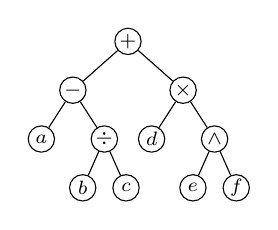
\begin{tikzpicture}[level distance=6.2mm,
 level 1/.style={sibling distance=14mm},
 level 2/.style={sibling distance=8mm},
 level 3/.style={sibling distance=5.5mm},
 every node/.style={circle,draw,inner sep=0.5pt,minimum size=9.5pt,font=\scriptsize}]
\node {$+$}
 child {node {$-$}
  child {node {$a$}}
  child {node {$\div$}
   child {node {$b$}}
   child {node {$c$}}}}
 child {node {$\times$}
  child {node {$d$}}
  child {node {$\wedge$}
   child {node {$e$}}
   child {node {$f$}}}};
\end{tikzpicture}
\end{center}
\begin{sloppypar}\raggedright
\textbf{Tree$\to$Lisp:} node $(op\ L\ R)$: \texttt{(+ (- a (/ b c)) (* d (\textasciicircum{} e f)))}.\\
\textbf{Lisp$\to$infix:} \texttt{(* (+ a b) c)} $\Rightarrow(a{+}b){\times}c$. Custom precedence $f(a,b){=}a\oplus b$: $f(f(x,y),z)$ parses as $x\oplus y\oplus z$; $f(x,f(y,z))$ as $x\oplus(y\oplus z)$ (structure differs).
\end{sloppypar}

\subsection{11--12. Transformations \& typed rewrite rules}
\begin{sloppypar}\raggedright
\textbf{Substitution} (replace a symbol/pattern everywhere): $x\to y{+}1$ in $x^2{+}2x{+}1$ $\Rightarrow(y{+}1)^2{+}2(y{+}1){+}1$.\\
\textbf{Expansion} (distribute, then combine): $(2x{+}3)(x{-}1)\to2x^2{-}2x{+}3x{-}3{=}2x^2{+}x{-}3$.\\
\textbf{Typed rule} $\frac{p::\mathrm{int}}{q::\mathrm{int}}\to\frac{p/g}{q/g}$ ($g{=}\gcd$): $\frac{6}{8}\to\frac34$ applies, $\frac{x}{y}$ does not ($x,y$ not ints).\\
\textbf{Combine like terms} ($c_1v{+}c_2v\to(c_1{+}c_2)v$ for variable $v$): $3x{+}5x\to8x$; $3x{+}5y$ matches no rule.
\end{sloppypar}

\subsection{13. Maxima (pseudocode only)}
\begin{sloppypar}\raggedright
Add two base-$B$ digit lists with carry: \texttt{for i:1 thru n do (s:l1[i]+l2[i]+c, r[i]:mod(s,B), c:floor(s/B))} $\Rightarrow$ result list $[r]$ plus final carry $c$. Digits are kept in $[0,B{-}1]$ by \texttt{mod}/\texttt{floor}.
\end{sloppypar}

\subsection{14--15. Modular arithmetic \& notation}
\begin{sloppypar}\raggedright
\textbf{Reduce first, then operate:} $34{+}29\equiv6{+}1{=}7\equiv0\pmod7$; $5{\cdot}6\equiv30\equiv2\pmod7$.\\
\textbf{Exponentiate with repeated reduction} (never the raw power): $3^4\bmod5$: $3^2{=}9\equiv4$, then $3^4\equiv4^2{=}16\equiv1$.\\
\textbf{Negative input:} $-17\bmod5$: add multiples of 5: $-17{+}20{=}3\Rightarrow-17\equiv3$.\\
\textbf{Notation:} $[12]_7{=}[5]_7\iff12\equiv5\pmod7$; $2{\cdot}3\equiv6\pmod7\iff[2]_7[3]_7{=}[6]_7$.
\end{sloppypar}

\subsection{16--17. Tables, inverses, zero divisors}
\begin{sloppypar}\raggedright
Build the $\times$-table mod $n$; row $a$ contains $1\iff a$ invertible; row $a$ has $0$ in a nonzero column $\Rightarrow a$ zero divisor.\\
Mod 6 (composite): row 2 $=0,2,4,0,2,4$ (no 1; $2{\cdot}3\equiv0$); row 3 $=0,3,0,3,0,3$; row 4 $=0,4,2,0,4,2$; row 5 $=0,5,4,3,2,1$ $\Rightarrow5^{-1}{=}5$ ($5{\cdot}5{=}25\equiv1$). Units: $\{1,5\}$.\\
Mod 5 (prime, all nonzero invertible): row 3 has 1 at col 2 $\Rightarrow3^{-1}{=}2$.
\end{sloppypar}

\subsection{18. Polynomial modular arithmetic (worked)}
\begin{sloppypar}\raggedright
\textbf{Reduce} mod $m(x)$ two ways: (A) use $m(x)\equiv0$ to eliminate powers; (B) \hl{long-divide} and keep the remainder (degree $<$ deg $m$). Mod $x^2{+}1$: $x^2\equiv-1$.\\
\textbf{(A)} $2x^3{+}x^2{-}3x{+}4$: $2x^3{=}2x{\cdot}x^2\equiv-2x$; $x^2\equiv-1$; so $\equiv-2x{-}1{-}3x{+}4{=}3{-}5x$ (class $[3-5x]$).\\
\textbf{(B) long division} of $x^3{+}2x^2{+}x{+}1$ by $x^2{+}1$:
\end{sloppypar}
\resizebox{0.86\linewidth}{!}{\polylongdiv[style=C]{x^3+2x^2+x+1}{x^2+1}}
\begin{sloppypar}\raggedright
$\Rightarrow$ quotient $x{+}2$, remainder $-1$; \hl{check} $(x{+}2)(x^2{+}1){+}(-1){=}x^3{+}2x^2{+}x{+}1$.\\
\textbf{Powers} (reduce at the end): $(1{+}x)^3{=}1{+}3x{+}3x^2{+}x^3\equiv1{+}3x{-}3{-}x{=}-2{+}2x$. Classes mod $x^2{+}1$ are all $a{+}bx$ (Gaussian integers $a{+}bi$).
\end{sloppypar}

\subsection{19. Inverse existence / zero divisors (theorem)}
\begin{sloppypar}\raggedright
\textbf{Theorem:} $m$ invertible mod $n\iff\gcd(m,n){=}1$; $n$ composite $\Rightarrow$ zero divisors exist.\\
$5$ mod $12$: $\gcd{=}1\Rightarrow$ invertible; $5^{-1}{=}5$ ($5{\cdot}5{=}25\equiv1$). $8$ mod $12$: $\gcd{=}4\ne1\Rightarrow$ \hl{no} inverse; zero divisor: $8{\cdot}3{=}24\equiv0$.\\
Mod 10: units $\{1,3,7,9\}$; $3^{-1}{=}7$ ($3{\cdot}7{=}21\equiv1$); zero divisors $4{\cdot}5{=}20\equiv0$, $6{\cdot}5{=}30\equiv0$.
\end{sloppypar}

\subsection{20--21. Groups: axioms \& multiplication tables}
\begin{sloppypar}\raggedright
\textbf{Verify ALL 4 axioms} (closure is the forgotten one). $(\mathbb Z_4,{+})$: closure ($[a]{+}[b]{=}[a{+}b]\in\mathbb Z_4$), identity $[0]$, inverse $[a]{+}[-a]{=}[0]$ (e.g. $[1]{+}[3]{=}[0]$, $[2]{+}[2]{=}[0]$), associative (integers) $\Rightarrow$ group.\\
$\mathbb Z_3^*{=}\{1,2\}$ table: $2{\cdot}2{=}4\equiv1$ $\Rightarrow$ rows $\{1,2\},\{2,1\}$; $1^{-1}{=}1$, $2^{-1}{=}2$; order-2 group.\\
$\mathbb Z_4^*{=}\{1,3\}$: $3{\cdot}3{=}9\equiv1$ $\Rightarrow$ group. $\{1,2,3\}$ with $\times$ mod 4 is \emph{not}: $2{\cdot}2{=}0\notin$ set (closure fails).
\end{sloppypar}

\subsection{22--23. Order, generator, Lagrange}
\begin{sloppypar}\raggedright
\textbf{Order:} smallest $n{>}0$ with $g^n{=}e$. Compute powers until $e$: in $\mathbb Z_7^*$: $2^1{=}2$, $2^2{=}4$, $2^3{=}8\equiv1$ $\Rightarrow\mathrm{ord}(2){=}3$.\\
\textbf{Generator} $\iff\mathrm{ord}(g){=}|G|$: $3$: powers $3,2,6,4,5,1$ (6 distinct) $\Rightarrow$ generator of $\mathbb Z_7^*$.\\
$\mathbb Z_{11}^*$ ($|G|{=}10$): $2$: $2,4,8,5,10,9,7,3,6,1\Rightarrow\mathrm{ord}{=}10\Rightarrow$ generator; $3$: $3,9,5,4,1\Rightarrow\mathrm{ord}{=}5$.\\
\textbf{Lagrange:} order divides $|G|$: $|\mathbb Z_{12}^*|{=}\varphi(12){=}4\Rightarrow$ orders $\in\{1,2,4\}$; $\varphi(9){=}6\Rightarrow\{1,2,3,6\}$.
\end{sloppypar}

\subsection{24. Fermat big powers}
\begin{sloppypar}\raggedright
\textbf{Method:} (1) check $p$ prime and $\gcd(a,p){=}1$; (2) $a^{p-1}\equiv1\pmod p$; (3) reduce base mod $p$; (4) $a^{(p-1)q{+}c}\equiv a^c$.\\
$3^{100}\bmod7$: $7$ prime, $7\nmid3$; $3^6\equiv1$; $100{=}6{\cdot}16{+}4$; $3^{100}\equiv3^4{=}81\equiv4$.\\
$5^{100}\bmod13$: $5^{12}\equiv1$; $100{=}12{\cdot}8{+}4$; $5^4{=}625\equiv1$. $2^{1000}\bmod7$: $1000{=}6{\cdot}166{+}4$; $2^4{=}16\equiv2$.
\end{sloppypar}

\subsection{25. Bases 16/8 (hex/octal) shortcuts}
\begin{sloppypar}\raggedright
\textbf{Dec$\to$hex:} same $\div16$ method, digits $0..9$,A,..,F: $45{=}2{\cdot}16{+}13\to0\mathrm{x}2D$. \hl{Check:} $2{\cdot}16{+}13{=}45$.\\
\textbf{Hex$\to$bin:} one hex digit $=$ 4 bits: $2D\to0010\ 1101{=}101101_2$; $111001_2\to0011\ 1001\to0\mathrm{x}39{=}57$.\\
\textbf{Hex$\to$dec:} $0\mathrm{x}2D{=}2{\cdot}16{+}13{=}45$. Group bits in 4s (hex) or 3s (octal) from the right.
\end{sloppypar}

\subsection{26. IEEE 754 special values}
\begin{sloppypar}\raggedright
Single (32-bit, bias 127): smallest positive normal $2^{-126}\approx1.17549{\times}10^{-38}$; largest normal $(2{-}2^{-23})2^{127}\approx3.40282{\times}10^{38}$.\\
24-bit float (bias 127, 7-bit exp, 16-bit mantissa): $E{=}e{+}127$; 16-bit course format $=$ bias 24, 5-bit exp, 10-bit mantissa (see \S35).
\end{sloppypar}

\subsection{27. LCM, more Euclid, base-$B$ practice}
\begin{sloppypar}\raggedright
$\mathrm{lcm}(a,b){=}\frac{ab}{\gcd(a,b)}$: $\mathrm{lcm}(12,18){=}\frac{216}{6}{=}36$. \\
Euclid again: $\gcd(84,30)$: $84{=}30{\cdot}2{+}24$, $30{=}24{\cdot}1{+}6$, $24{=}6{\cdot}4{+}0\Rightarrow\gcd{=}6$.\\
Base-60: $3601{=}[1,0,1]_{60}$ ($60^2{+}1$), $125{=}[0,2,5]_{60}$; sum $[1,2,6]_{60}{=}3600{+}120{+}6{=}3726$ ($3601{+}125$).\\
\end{sloppypar}

\subsection{28. More trees \& rewrites}
\begin{sloppypar}\raggedright
$a{\cdot}(b{+}c)-d$: root $-$, left $\times$, right $d$; Lisp: \texttt{(- (* a (+ b c)) d)}.\\
Substitute $z{=}x{+}y$ in $z^2{-}1$: $\Rightarrow(x{+}y)^2{-}1$; expand $(x{+}y)^2{=}x^2{+}2xy{+}y^2$.\\
Rule $c_1v^2{+}c_2v^2\to(c_1{+}c_2)v^2$: $2x^2{+}3x^2\to5x^2$; $2x^2{+}3y^2$ no match ($x\ne y$).
\end{sloppypar}

\subsection{29. Solving simple linear congruences}
\begin{sloppypar}\raggedright
\textbf{Solve $ax\equiv b\pmod n$:} if $\gcd(a,n)\nmid b$ no solution; divide all three by $\gcd$; multiply by $a^{-1}$.\\
$3x\equiv1\pmod7$: $\gcd(3,7){=}1$; $3^{-1}{=}5$ ($3{\cdot}5{=}15\equiv1$); $x\equiv5\pmod7$.\\
$4x\equiv2\pmod6$: $\gcd(4,6){=}2$ divides $2\Rightarrow2$ solutions; divide: $2x\equiv1\pmod3$; $2^{-1}{=}2$; $x\equiv2\pmod3\Rightarrow x{=}2,5$ (check $4{\cdot}2{=}8\equiv2$, $4{\cdot}5{=}20\equiv2$).
\end{sloppypar}

\subsection{30. More generators \& orders}
\begin{sloppypar}\raggedright
$\mathbb Z_{13}^*$ ($|G|{=}12$): powers of 2: $2,4,8,3,6,12,11,9,5,10,7,1$ $\Rightarrow\mathrm{ord}(2){=}12\Rightarrow$ generator.\\
$\mathbb Z_7^*$: $\mathrm{ord}(2){=}3$, $\mathrm{ord}(3){=}\mathrm{ord}(5){=}6$, $\mathrm{ord}(4){=}3$, $\mathrm{ord}(6){=}2$; generators $=\{3,5\}$.\\
$\mathbb Z_{11}^*$ ($|G|{=}10$): generators $=\{2,6,7,8\}$. $\mathbb Z_8^+$: $[1],[3],[5],[7]$ order 8; $[2],[6]$ order 4; $[4]$ order 2. \hl{Cyclic} $\iff\exists g$ with $\mathrm{ord}(g){=}|G|$.
\end{sloppypar}

\subsection{31. More Fermat practice}
\begin{sloppypar}\raggedright
$3^{49}\bmod7$: $3^6\equiv1$; $49{=}6{\cdot}8{+}1$; $3^{49}\equiv3^1{=}3$.\\
$11^{1000}\bmod17$: $11^{16}\equiv1$; $1000{=}16{\cdot}62{+}8$; $11^8{=}(11^2)^4{=}(121\equiv2)^4{=}16\equiv-1\Rightarrow11^{1000}\equiv16$.\\
$2^{200}\bmod31$: $2^{30}\equiv1$; $200{=}30{\cdot}6{+}20$; $2^{20}{=}(2^5)^4{=}32^4\equiv1$. \hl{Shortcut} if base $\equiv0$: $21^{50}\bmod7{=}0$.\\
\textbf{Mod-6 $\times$ table} (read off inverses \& zero divisors):\\
${\renewcommand{\arraystretch}{0.88}\begin{array}{c|cccccc}\times&0&1&2&3&4&5\\\hline0&0&0&0&0&0&0\\1&0&1&2&3&4&5\\2&0&2&4&0&2&4\\3&0&3&0&3&0&3\\4&0&4&2&0&4&2\\5&0&5&4&3&2&1\end{array}}$
$\quad$ Row 5 has a 1 (col 5) $\Rightarrow5^{-1}{=}5$; rows 2,3,4 hit 0 $\Rightarrow$ zero divisors. Units $\{1,5\}$.
\end{sloppypar}

\subsection{32. Signed overflow (two's complement)}
\begin{sloppypar}\raggedright
\textbf{Add two positives and get a negative (or vice-versa) $\Rightarrow$ overflow.} 8-bit: $127{+}1$: $01111111{+}00000001{=}10000000{=}-128$ (overflow!); $100{+}100{=}200>127$ also overflows. \hl{Trap:} $-128$ has no positive twin.
\end{sloppypar}

\subsection{33. Constructing the $D_3$ table}
\begin{sloppypar}\raggedright
Relations: $r^3{=}e$, $\ell_i^2{=}e$; $r{\circ}\ell_1{=}\ell_2$, $r^2{\circ}\ell_1{=}\ell_3$; entry $=$ \hl{column first, then row}.\\
Row $r$: $r{\circ}e{=}r$, $r{\circ}r{=}r^2$, $r{\circ}r^2{=}e$, $r{\circ}\ell_1{=}\ell_2$, $r{\circ}\ell_2{=}\ell_3$, $r{\circ}\ell_3{=}\ell_1$; \hl{check:} each row is a permutation of all 6 (Latin square). $r^{-1}{=}r^2$, $\ell_i^{-1}{=}\ell_i$.
\end{sloppypar}

\subsection{34. Constructing a $+$ table mod $n$}
\begin{sloppypar}\raggedright
\textbf{Row $a$ of the $+$-table} $=$ row 1 shifted cyclically by $a$: mod 7, row 1 $=0,1,2,3,4,5,6$; row 3 $=3,4,5,6,0,1,2$. $[a]+[b]=[a{+}b\bmod n]$. \hl{Additive inverse} $[-a]=[n-a]$: mod 7, $[3]^{-1}{=}[4]$; mod 6, $[2]^{-1}{=}[4]$, $[5]^{-1}{=}[1]$.
\end{sloppypar}

\subsection{35. IEEE 754 16-bit (course: bias 24) worked}
\begin{sloppypar}\raggedright
\textbf{Convert $2.5$} (5-bit exp, 10-bit mantissa, bias 24): $2.5{=}10.1_2{=}1.01_2{\times}2^1$; $s{=}0$; $f{=}01$ padded to 10 bits; $E{=}1{+}24{=}25{=}11001_2$ $\Rightarrow$ bits $0\ 11001\ 0100000000$.\\
\textbf{Decode:} $E{=}25\Rightarrow e{=}1$; $(1.01)_2{=}1.25$; $1.25{\times}2{=}2.5$. \hl{Check:} $\max{=}(2{-}2^{-10})2^{31-24}{=}255.875$.
\end{sloppypar}

\subsection{36. APN multiplication (schoolbook)}
\begin{sloppypar}\raggedright
Multiply digit lists base $B$: each digit pair $a_i b_j$ adds to position $i{+}j$, carrying down. $[4,2]\times[3,1]$ base 10 ($24{\times}13{=}312$): units $4{\cdot}3{=}12\to$ digit $2$, carry $1$; then $4{\cdot}1{+}2{\cdot}3{+}1{=}11\to$ digit $1$, carry $1$; then $2{\cdot}1{+}1{=}3$. Result $[2,1,3]{=}312$.
\end{sloppypar}

\textbf{Quick Reference:} Powers of 2: $2^{10}=1024$, $2^{11}=2048$, $2^{20}\approx10^6$, $2^{31}\approx2.147{\times}10^9$, $2^{63}\approx9.22{\times}10^{18}$. $\sqrt2\approx1.41421$, $\sqrt3\approx1.73205$, $\pi\approx3.14159$, $e\approx2.71828$, $\ln6\approx1.79176$. $7!=5040$, $8!=40320$, $10!=3628800$. $\frac9{11}=0.(81)$, $\frac13=0.(3)$, $0.1_{10}=0.0\overline{0011}_2$.

\end{multicols}
\end{document}